% Chapter Template

\chapter{Classical numerical results} % Main chapter title

\label{Chapter3} % Change X to a consecutive number; for referencing this chapter elsewhere, use \ref{ChapterX}


%----------------------------------------------------------------------------------------
%	SECTION 1
%----------------------------------------------------------------------------------------

In this section we will revisit the two classical results in computational finance, which is the Binomial model and the Least Square Monte Carlo (LSM) approach. The models will both serve as reference for the Machine Learning model and provides different insight into valuation of American options.


\section{Binomial Pricing model}
The Binomial model provides an intuitive and easy implementable model for valuing american and european options. The Binomial model comes handy, when no analytical model exists for american options. The Binomail model also has its limitations, because it is not suited for valuing path dependent options or options with several underlying factors. The key difference on the Binomial model and the other numerical procudures is that the Binomial model is build on a discrete framework. \\

The central concepts arbitrage and completeness from continuous time also work in the discrete time setup. The paper \parencite{binomial-Paper} which introduced the binomial model to option pricing came after the Black-Scholes model described in section \ref{Chapter2} \parencite{B-S-Paper}. The main reason for develop a model in discreste time, is that the the discrete time approach gives a simplified model in terms of the mathematics and highlights the essential concepts in option pricing theory arbitrage and hedging. You can argue that the simpler mathematics in this model makes the binomial model more instructive and clear from an economist viewpoint. Besides being easier to understand for non-mathematician it works nicely with other options than the European options like American options. It serves also as a comparision for the other algorithm's. The model gives a instructive way of thinking about arbitrage and hedging. \\

Eventhough we assume the stock price moves at discrete time instead of continuous time. We
It can actually be shown that if you choose your parameters in this model to follow the mean and variance in the continuous time framework then the discrete time model will converge to the continuous time model \parencite{binomial-Paper}. Hence the binomial pricing model will be equivalent with the continuos time analytical pricing model derived by Fischer Black and Myron Scholes in the limit for european options \parencite{binomial-Paper}.\\

To value a american put option, we lay out all the possible path of the stock, based on the $S_0, K, \sigma, r, T$. We also need to specify the number of steps for the tree, where for each step, we add another possible value for the stock. We only add 1 more possibility because the tree recombines. The precision for the algorithme increases with the number of steps and the option value converge to a value (see Figure \ref{fig:binConv}). For valuing an american put option, we value the exercise value at maturity (time T) for all possible outcomes for the stock. Then we work backward in the tree by comparing intrinsic value with the conditional expectation, where we choose the maximum of these two \parencite{Hull}. 
 
\begin{figure}[th]
\centering
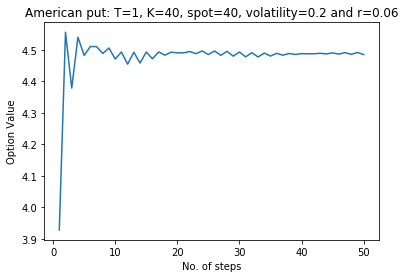
\includegraphics{Figures/binConv.png}
\decoRule
\caption[Convergence of Binomial model]{}
\label{fig:binConv}
\end{figure}



%-----------------------------------
%	SUBSECTION 1
%-----------------------------------
\subsection{Mathematics in binomial model}
The mathematics behind the binomial model are simpel and we will this section to provide the basic.
We assume the stock S can move up (u) or down (d) with probability p. In order to avoid arbitrage, we need to change the measure to the EMM Q. To calculate Q we set up a portfolio with no risk, so we expect the risk free rate R. We zoom in into a single timestep to simplify even futher and it can easily be generalizes to multiple timesteps.

\subsubsection{1-time period binomial model}
We calculate q by\\
111111111
\begin{equation}
\begin{split}
S_0=\frac{1}{1+R} E^Q[S_1]=\frac{1}{1+R} (p\cdot S_0 u + (1-p) S_0 d)\\
\Rightarrow 1+R=p(u-d)+d \Rightarrow \frac{1+R-d}{u-d}  
\end{split}
\end{equation} 
!!!!!!!!!!!

Now that we have the risk neutral probabilities, we can easily work backward in the tree by $max\{ K-S, e^{-R \Delta t} (q\cdot Su, (1-q)\cdot Sd) \}$. We we work all the way back to the root, we get the value of the american put option.

%-----------------------------------
%	SUBSECTION 2
%-----------------------------------


%----------------------------------------------------------------------------------------
%	SECTION 2
%----------------------------------------------------------------------------------------

\section{Least Square Monte Carlo Method}
The other classical result in this section is somewhat more technical without familarity with statistics, but on the other hand the least square method and linear regression is a well known and testet in statistics. In our setting we regress the expected payoff by continuation of the contract and compare it to the intrinsic value. The dependent variable is the expected value and the independent variables is a set of othogonal basis functions in $L^2(\Omega, \mathcal{F}, Q)$. Typical choices for basis functions could be weighted Laguerre -, Hermit -, and Jacob polynomials. This kind of regression is a nonlinear expansion of the linear model. In order to create data, we will simulate paths according to the underlying risky asset. 

\subsection{Application of the LSM method}
We want to valuate an American put option with a stock as underlying asset. We assume the stock follows a GBM: $dS(t)=rSdt + \sigma S dW_t$ where $\sigma$ and r is constant (see solution to SDE equation \ref{GBM}). We simulate 100.000 paths for the stock, where 50.000 of the paths is antithetic of the first 50.000 using 50 exercise points per year.

\parencite{lsm}  

\section{Comparision}

